\section{Les pratiques du développeur}
\label{sec:pratiques}

% Réutilisation, Encapsulation maximale, Couplage faible, Cohésion forte, DRY, KISS, YAGNI
% Loi de demeter
% SOLID
% Commentaire, formattage, langue, nommage

\lstset{basicstyle=\ttfamily\tiny}

\begin{frame}
    \frametitle{SOLID}

    \begin{columns}
        \begin{column}{0.5\textwidth}
            \begin{itemize}
                \item Principe de responsabilité unique
                \item Principe ouvert/fermé
                \item Principe de substitution de Liskov
                \item Principe de ségrégation des interfaces
                \item Principe d'inversion des dépendances
            \end{itemize}
        \end{column}
        \begin{column}{0.5\textwidth}
            \begin{itemize}
                \item Single Responsibility Principle
                \item Open/closed principle
                \item Liskov substitution principle
                \item Interface segregation principle
                \item Dependency inversion principle
            \end{itemize}
        \end{column}
    \end{columns}
\end{frame}

\begin{frame}
    \frametitle{Principe de responsabilité unique}

    \begin{columns}
        \begin{column}{0.5\textwidth}
            \lstinputlisting[
                language={[Sharp]C},
                label=lst:srp-ko]
            {figures/pratiques/srp-ko.cs}
        \end{column}
        \pause
        \begin{column}{0.5\textwidth}
            \lstinputlisting[
                language={[Sharp]C},
                label=lst:srp-ok]
            {figures/pratiques/srp-ok.cs}
        \end{column}
    \end{columns}
\end{frame}

\begin{frame}
    \frametitle{Principe de responsabilité unique}

    Une classe doit avoir une et une seule raison de changer !

    \begin{itemize}
        \item La classe est plus facile à comprendre ;
        \item La classe est plus facile à maintenir ;
        \item La classe est plus réutilisable.
    \end{itemize}

    \bigskip
    Le SRP équivaut à peu près à avoir une \textbf{« cohésion élevée »}.
    On dit qu’une classe a une forte cohésion si ses comportements sont fortement liés et fortement concentrés.
    Le SRP stipule qu’une classe doit être cohérente au point d’avoir une seule responsabilité,
    où une responsabilité est définie comme \textbf{« une raison de changement »}.

\end{frame}

\begin{frame}
    \frametitle{Principe ouvert/fermé}

    \begin{columns}
        \begin{column}{0.5\textwidth}
            \lstinputlisting[
                language={[Sharp]C},
                label=lst:ocp-ko]
            {figures/pratiques/ocp-ko.cs}
        \end{column}
        \pause
        \begin{column}{0.5\textwidth}
            \lstinputlisting[
                language={[Sharp]C},
                label=lst:ocp-ok]
            {figures/pratiques/ocp-ok.cs}
        \end{column}
    \end{columns}
\end{frame}


\begin{frame}
    \frametitle{Principe ouvert/fermé}

    Vous devriez pouvoir étendre le comportement d'une classe, sans le modifier.\\
    Une classe doit être ouverte à l’extension, mais fermée à la modification.

    \begin{itemize}
        \item La classe devient robuste, flexible et réutilisable ;
        \item Moins de modification implique moins de bogue.
    \end{itemize}

\end{frame}

\begin{frame}
    \frametitle{Principe de substitution de Liskov}

    \begin{columns}
        \begin{column}{0.5\textwidth}
            \lstinputlisting[
                language={[Sharp]C},
                label=lst:lsp-ko]
            {figures/pratiques/lsp-ko.cs}
        \end{column}
        \pause
        \begin{column}{0.5\textwidth}
            \lstinputlisting[
                language={[Sharp]C},
                label=lst:lsp-ok]
            {figures/pratiques/lsp-ok.cs}
        \end{column}
    \end{columns}
\end{frame}

\begin{frame}
    \frametitle{Principe de substitution de Liskov}

    Les fonctions qui utilisent une classe de base doivent
    pouvoir utiliser des objets de classes dérivées sans le savoir.

    Lorsque les sous-classes n'adhèrent pas correctement à l'interface de la classe de base,
    il faut parcourir le code existant et tenir compte des cas particuliers impliquant les sous-classes délinquantes.
    Il s’agit d’une violation flagrante du principe ouvert/fermé.

    \bigskip
    Lors de l’apprentissage de la programmation orientée objet,
    l’héritage est généralement décrit comme une relation « est un »,
    mais elle entraîne \textbf{parfois une mauvaise utilisation de l'héritage}.

\end{frame}

\begin{frame}
    \frametitle{Principe de ségrégation des interfaces}

    \begin{columns}
        \begin{column}{0.5\textwidth}
            \lstinputlisting[
                language={[Sharp]C},
                label=lst:isp-ko]
            {figures/pratiques/isp-ko.cs}
        \end{column}
        \pause
        \begin{column}{0.5\textwidth}
            \lstinputlisting[
                language={[Sharp]C},
                label=lst:isp-ok]
            {figures/pratiques/isp-ok.cs}
        \end{column}
    \end{columns}
\end{frame}

\begin{frame}
    \frametitle{Principe de ségrégation des interfaces}

    Les clients ne devraient pas être obligés de dépendre d’interfaces qu’ils n’utilisent pas.

    Ce principe permet d'éviter le couplage involontaire entre classes.
\end{frame}

\begin{frame}
    \frametitle{ISP, OCP, and DIP… OMG WTF BBQ?}

    L'exemple précédent ne viole pas simplement la ségrégation des interfaces (ISP),
    il viole également inversion de dépendance (DIP) et le principe d'ouverture/fermeture (OCP).
    C’est assez courant, donc si vous adhérez correctement au DIP et à l’OCP,
    vous ne rencontrerez pas de nombreuses violations de l'ISP.
    Cela dit, c'est un autre moyen pratique d'évaluer la conception de votre classe.

    \bigskip
    \textbf{``Ai-je besoin de toutes les méthodes de cette interface que j'utilise ?''}

    Si la réponse est non, vous souhaiterez peut-être utiliser une interface différente
    et appliquer certains des autres principes SOLID.
\end{frame}

\begin{frame}
    \frametitle{Principe d'inversion des dépendances}

    \begin{columns}
        \begin{column}{0.5\textwidth}
            \lstinputlisting[
                language={[Sharp]C},
                label=lst:dip-ko]
            {figures/pratiques/dip-ko.cs}
        \end{column}
        \pause
        \begin{column}{0.5\textwidth}
            \lstinputlisting[
                language={[Sharp]C},
                label=lst:dip-ok]
            {figures/pratiques/dip-ok.cs}
        \end{column}
    \end{columns}
\end{frame}

\begin{frame}
    \frametitle{Principe d'inversion des dépendances}

    Les modules de haut niveau ne doivent pas dépendre de modules de bas niveau.
    Les deux devraient dépendre d’abstractions.

    Ce principe permet de réduire le couplage entre composants.

    \bigskip
    Le principe d'inversion de dépendance est essentiellement un moyen d'ajouter des fiches et des prises à votre code.
    Il vous permet de créer des modules de haut niveau indépendants des modules de bas niveau.
    Les modules de bas niveau peuvent être créés ultérieurement et sont facilement remplaçables.
\end{frame}

\begin{frame}
    \frametitle{SOLID}

    \centering
    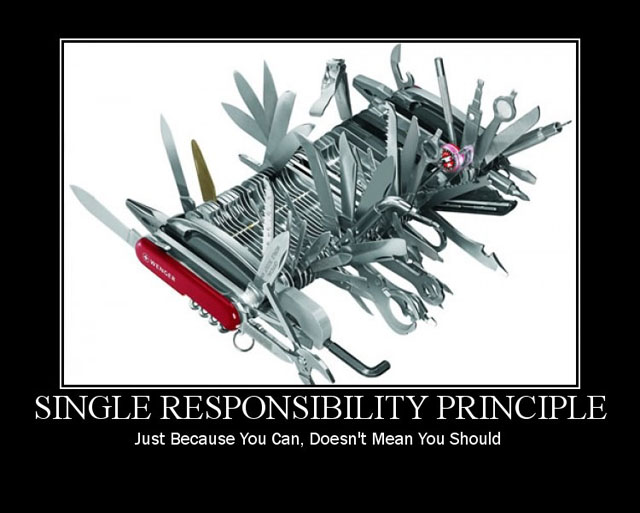
\includegraphics[height=100px]{figures/pratiques/srp}
    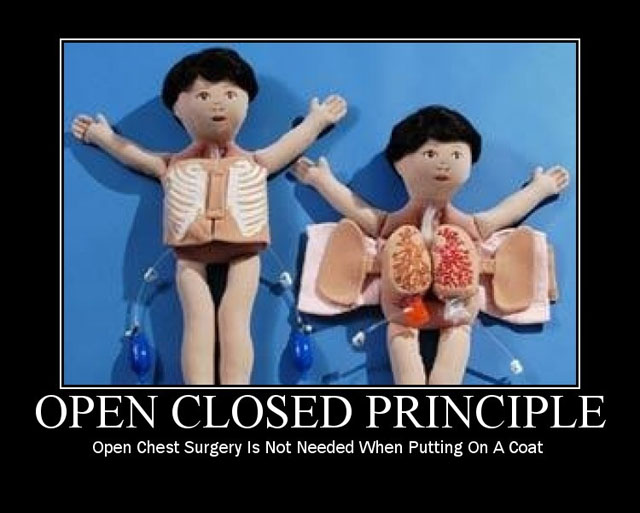
\includegraphics[height=100px]{figures/pratiques/ocp}
    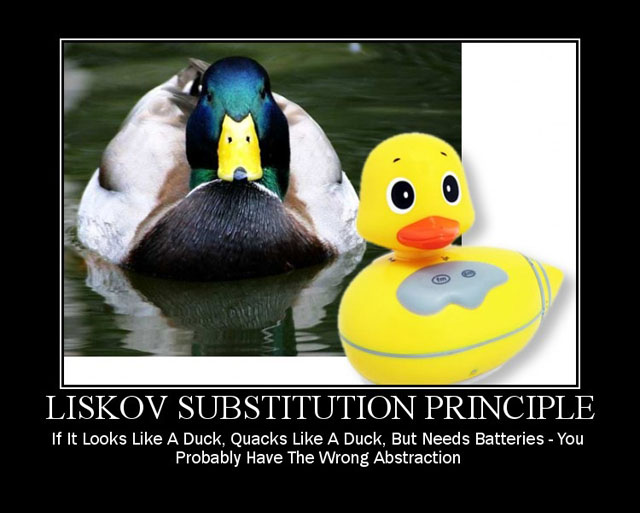
\includegraphics[height=100px]{figures/pratiques/lsp}

    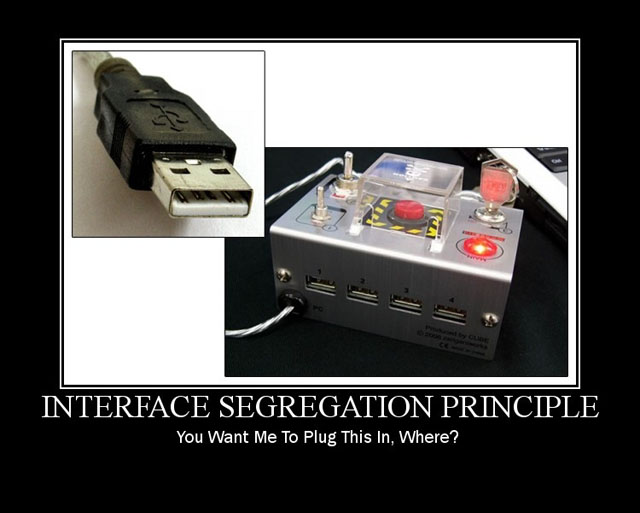
\includegraphics[height=100px]{figures/pratiques/isp}
    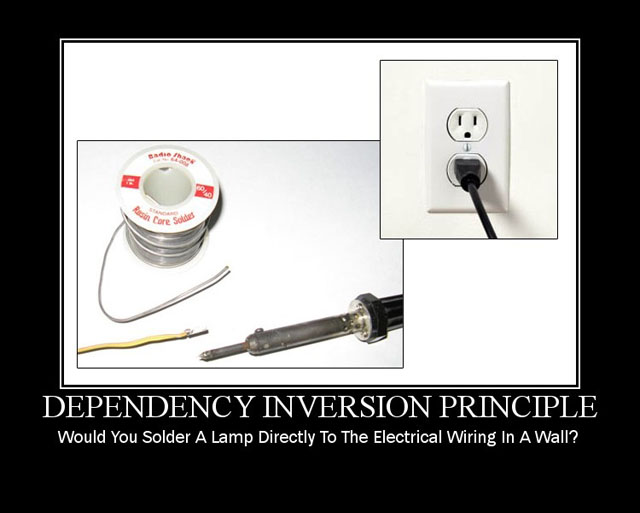
\includegraphics[height=100px]{figures/pratiques/dip}

\end{frame}

\begin{frame}
    \centering
    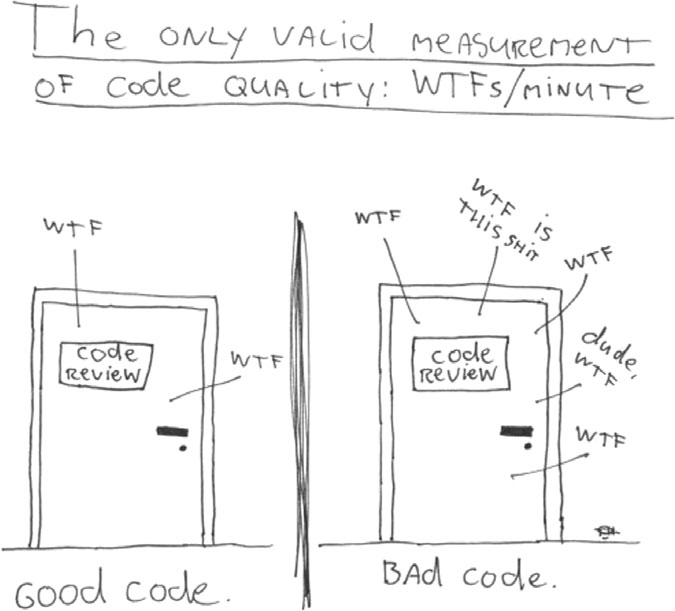
\includegraphics[height=0.5\linewidth]{figures/pratiques/wtf}
\end{frame}
